\documentclass{beamer}
\usetheme{}
\usecolortheme{dolphin}           
\useinnertheme{circles}
\setbeamertemplate{itemize items}[default]
\setbeamertemplate{enumerate items}[default]
\usepackage[T1]{fontenc}
\usepackage[utf8]{inputenc}
\usepackage{lmodern}
\usepackage{amsmath}
\usepackage{booktabs} 
\usepackage{graphicx}        
\usepackage{array}
\usepackage{color}
\usepackage{svg}
\makeatletter
\def\zapcolorreset{\let\reset@color\relax\ignorespaces}
\def\colorrows#1{\noalign{\aftergroup\zapcolorreset#1}\ignorespaces}
\makeatother
\graphicspath{{/home/swl/Dropbox/ucd/advanced_macro/figures/}} 
\setbeamertemplate{navigation symbols}{}
%--------------------------------------
%%%% DETAILS TITLE PAGE %%%%
%--------------------------------------
\title{Identification in macroeconomics}
\author{School of Economics, University College Dublin}
\date{Spring 2018}
\begin{document}

%--------------------------------------
\begin{frame}
 \titlepage
\end{frame}
%--------------------------------------

%--------------------------------------
\begin{frame}
  In general macroeconometricians do four things
  \begin{enumerate}
    \item Describe and summarise macroeconomic data
    \item Make macroeconomic forecasts
    \item Quantify what we - don't- know about the macroeconomy
    \item Advise policymakers - on macroeconomic issues
  \end{enumerate}
\end{frame}
%--------------------------------------

%--------------------------------------
\begin{frame}
 In terms of empirical research, some of the most important questions in macroeconomics are  
  \begin{itemize}
    \item Why do some countries grow faster than others?
    \medskip
    \item What causes business cycle fluctuations?
    \item How does monetary or fiscal policy affect the economy?    
  \end{itemize}    
\end{frame}
%--------------------------------------

%--------------------------------------
\begin{frame}
  Often answers to macroeconomic questions are 
  \begin{enumerate}
    \item Unknown
    \item Difficult to answer
  \end{enumerate}
  \medskip
  A major complication - as in any empirical field - is identification.
\end{frame}
%--------------------------------------

%--------------------------------------
\begin{frame}
  What is identification?
  \begin{itemize}
    \item Necessary condition for the existence of consistent estimators
    \item i.e. when sample size increases, the estimator will converge, probabilistically, to parameters unknown value
  \end{itemize}
  \medskip
  Analytically, identification entails whether or not the unknown parameter value can be deduced from the observed data
  \begin{itemize}
    \item Consistent estimators may exist under number of assumptions, i.e. central limit theorem etc.
  \end{itemize}
\end{frame}
%--------------------------------------

%--------------------------------------
\begin{frame}
  Let's consider an example looking at the FED interest rates:
  In 2008 the FED lowered the rates in a reaction to the crisis.
  \begin{itemize}
    \item Lowering interest rates should encourage spending; stimulate economic activity
  \end{itemize}
  \medskip
  Changes in interest rate are a source of variation in monetary policy which can be used in the model. 
\end{frame}
%--------------------------------------

%--------------------------------------
\begin{frame}
  \begin{figure}
    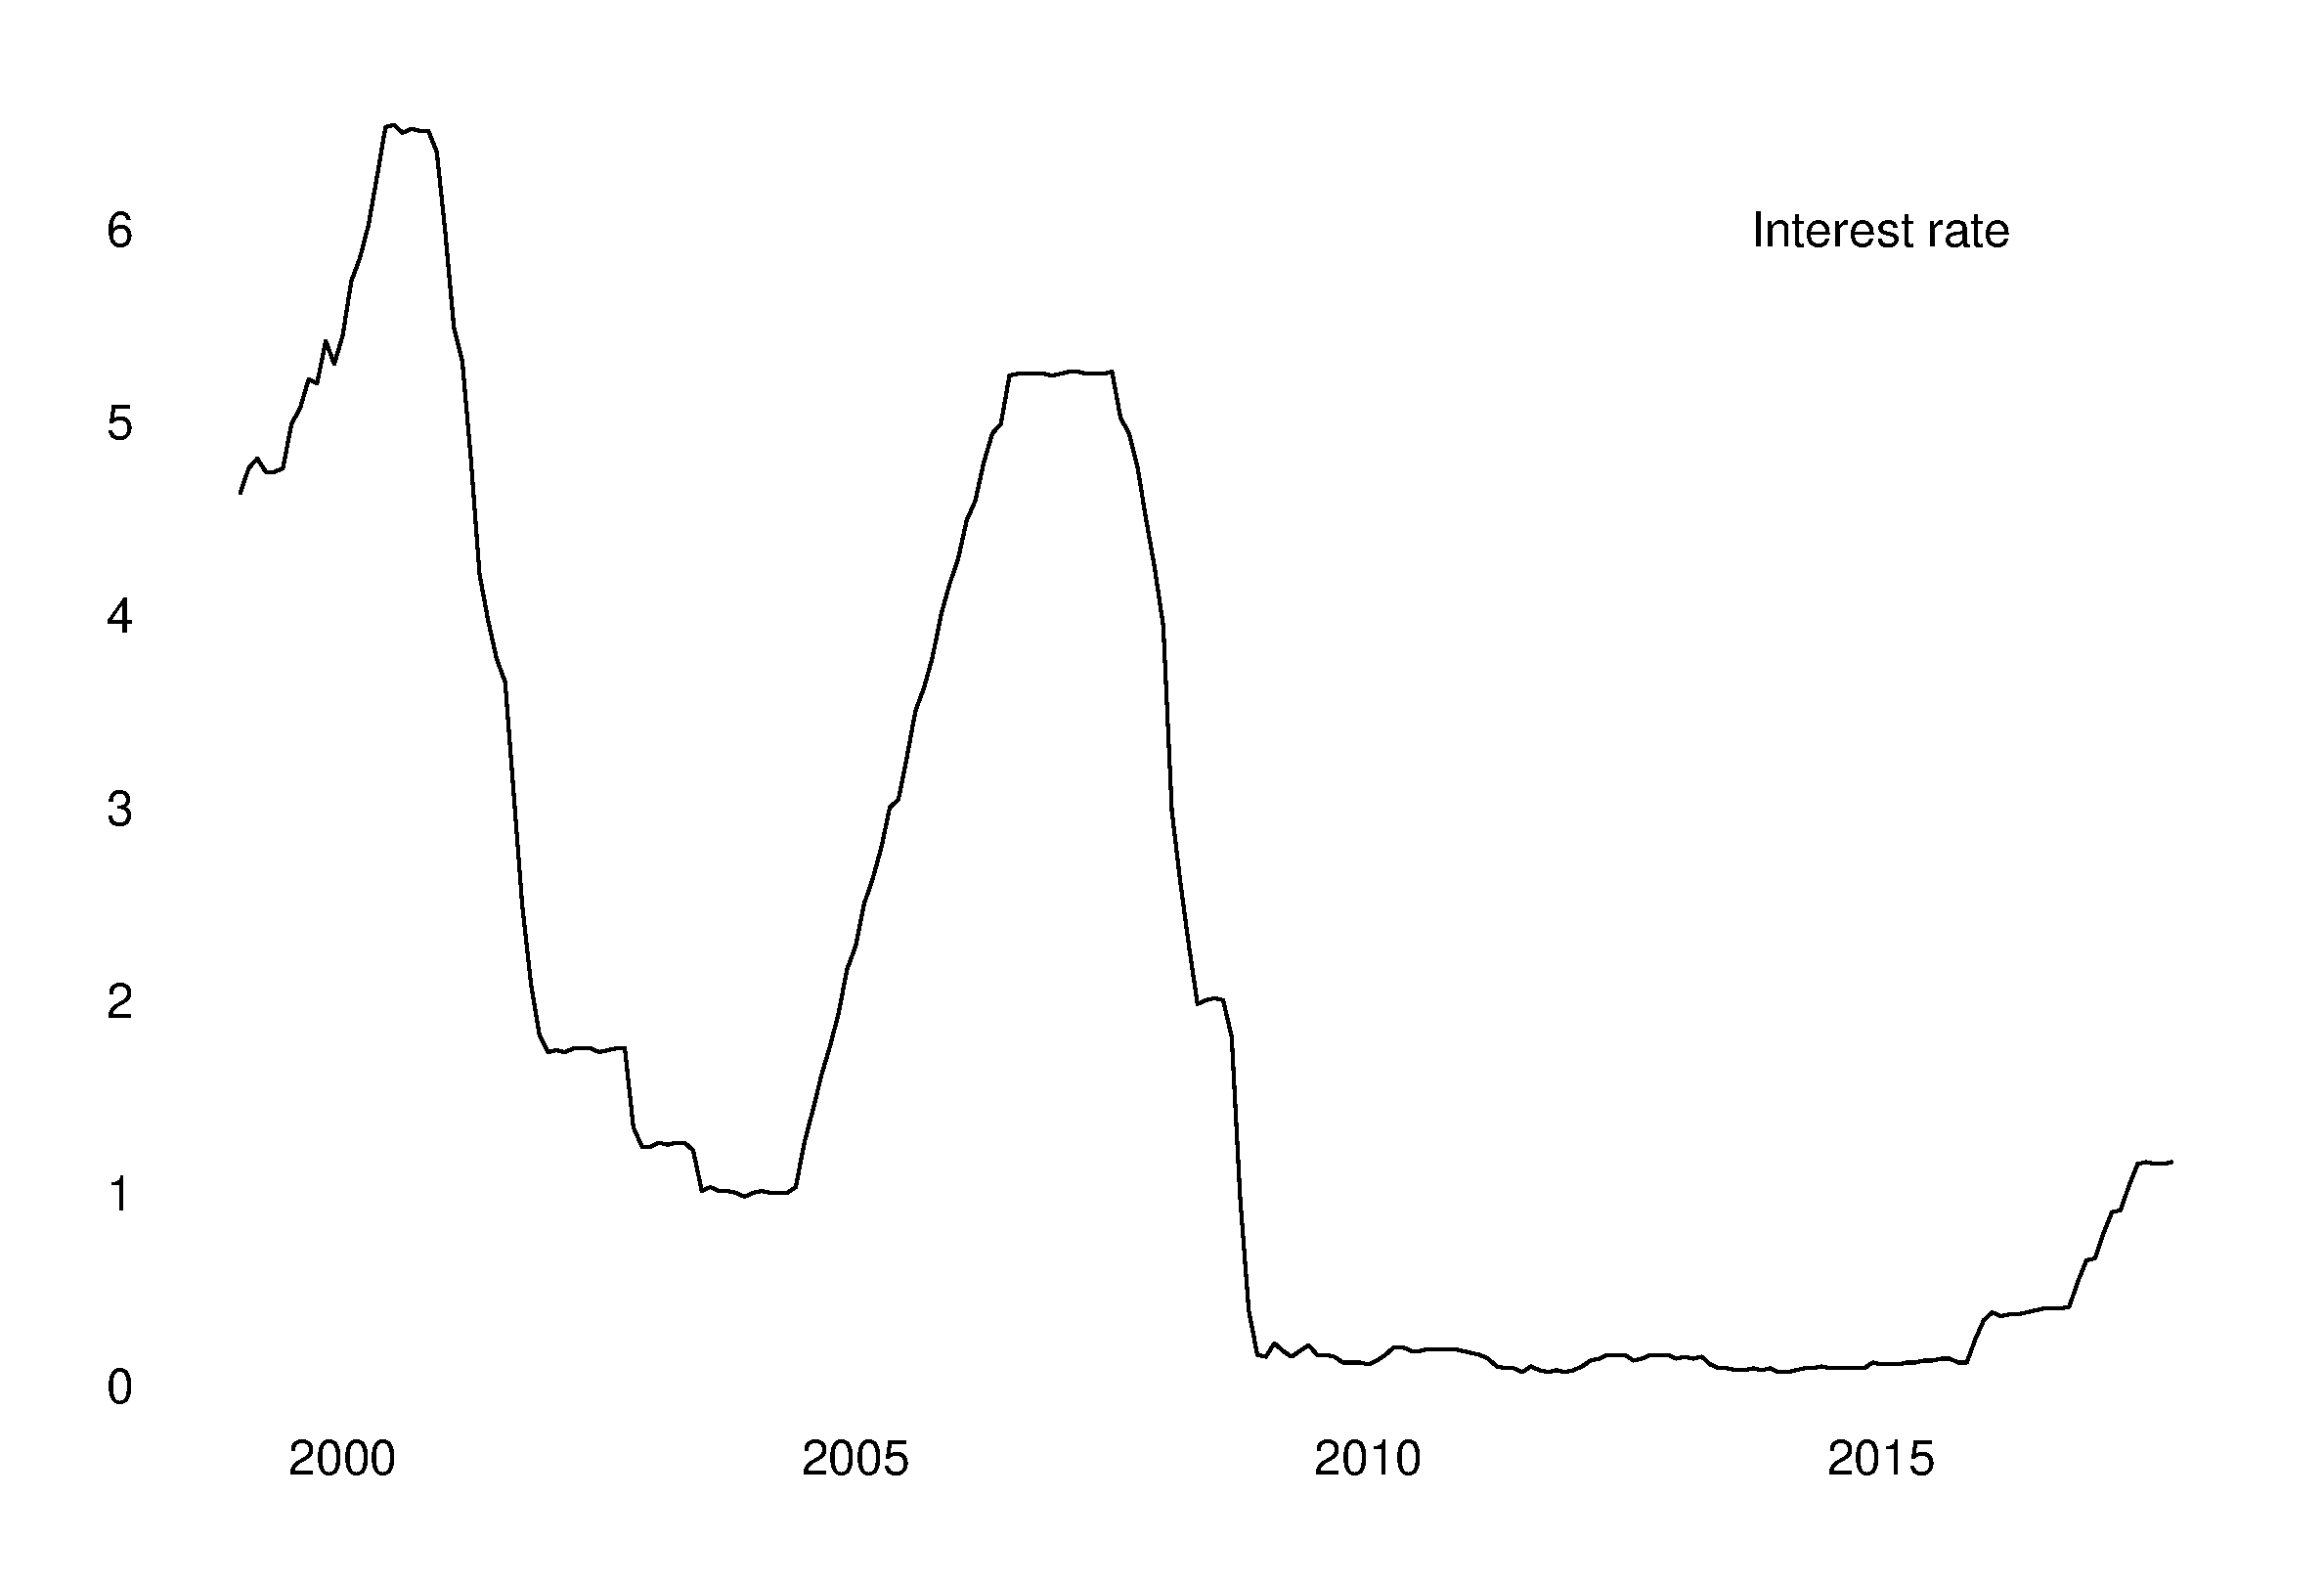
\includegraphics[scale=.3]{effective_rate.eps}
  \end{figure}
\end{frame}
%--------------------------------------

%--------------------------------------
\begin{frame}
 Can estimate effect of interest rate on economic output using following model: 
  \begin{align*}
    \Delta GDP_t = \alpha + \beta \Delta i_t + \epsilon_t
  \end{align*}
  \medskip
  Estimate using OLS, possible estimate: $\beta > 0$
\end{frame}
%--------------------------------------


%--------------------------------------
\begin{frame}
  Simple OLS regression would lead to conclusion that reduction in interest rate correlates/causes decreases in output
  \begin{itemize}
    \item Lowering interest rate harms the economy
  \end{itemize}
  \medskip
  Policy implication would be to increase interest rates to stimulate economic activity.
  \begin{itemize}
    \item Sticking to evidence-based policy
  \end{itemize}
\end{frame}
%--------------------------------------

%--------------------------------------
\begin{frame}
  FED does not change interest rates randomly
  \begin{itemize}
    \item Interest rates are endogenous    
  \end{itemize}
  \medskip
  Interest rates are lowered because some factors affect economy negatively
  \begin{itemize}
    \item Around 2008 think falling house prices and their effect on bank balance sheets
  \end{itemize}
  \medskip
  These other factors confound effect of change in monetary policy
  \begin{itemize}
    \item i.e. OLS regression does not capture isolated effect of interest rate
  \end{itemize}
\end{frame}
%--------------------------------------

%--------------------------------------
\begin{frame}
  Paramount in macroeconomic research is the role of dynamics, and there are two important challenges:
  \begin{enumerate}
    \item Difficult to identify exogenous variation in macroeconomic policy
    \item Natural experiment that can be identified are rarely those required to answer questions we're interested in. 
  \end{enumerate}
  \medskip
  As a result, there is an external validity problem.
\end{frame}
%--------------------------------------


%--------------------------------------
\begin{frame}
 There are some additional important issues : 
 \begin{enumerate}
   \item Dynamic nature of monetary and fiscal policy make it high dimensional; can have effect on both short and long run
   \item Effects of fiscal shocks depends on monetary policy (constrained by zero lower bound) and tax policy response
   \item Effect of policy depends on the economy
   \item Degree to which a policy is a surprise affects when and how strongly an economy reacts  
 \end{enumerate}
 \medskip
 This entails that macroeconomic research tends to be structural in nature
 \begin{itemize}
   \item Different from other empirical economic research which seeks to identify causal effects
 \end{itemize} 
\end{frame}
%--------------------------------------

%--------------------------------------
\begin{frame}
  As in any quantitative field macroeconomics relies on the use of statistical methods and thus on the use of moments
  \begin{itemize}
    \item Moments characterises the statistical distribution and are most commonly taken around the mean
  \end{itemize}
  \medskip
  In terms of econometrics we can distinguish between identified and unidentified moments
  \begin{enumerate}
    \item Unidentified: simple statistics such as means, variances, and correlations
    \item Identified: Statistics derived from empirical strategies or causal effect estimates 
  \end{enumerate}
\end{frame}
%--------------------------------------

%--------------------------------------
\begin{frame}
 Identified moments are designed to help uncover causal effects (micro) or responses to structural shocks (macro).
 \begin{enumerate}
   \item Micro moments are constructed using microeconomic data on behaviour of individuals and firms
   \item Macro moments use aggregated data to identify equilibrium outcomes; informative about what type of world we live in 
  \end{enumerate} 
\end{frame}
%--------------------------------------

%--------------------------------------
\begin{frame}
  Do identified moments correspond to structural parameters?
  \begin{itemize}
    \item They do in some cases: Labour supply elasticity in labour economics
  \end{itemize}
  \medskip
  In other cases they don't
  \begin{enumerate}
    \item Marginal propensity to consume following transitory fiscal rebate
    \item Estimate of regional fiscal multiplier
  \end{enumerate}
  \medskip
  In cases where they don't correspond you need a theoretical framework to go from the identified moments to the macroeconomic question of interest.
\end{frame}
%--------------------------------------

%--------------------------------------
\begin{frame}
 Finally there is the issue of data and the unit-of-analysis which means that identification can be done at
  \begin{enumerate}
    \item Aggregate level; focusing on single country
    \item Cross-sectional level; e.g. across countries or within country
  \end{enumerate}
  \medskip
  Cross-sectional identification is a fairly recent development
  \begin{itemize}
    \item Due to improvements in data collection
    \item Cross-sectional identification brings additional estimation challenges
  \end{itemize}
\end{frame}
%--------------------------------------

%--------------------------------------
\begin{frame}
 Majority of studies are based on U.S. economy
 \begin{itemize}
   \item Largest economy in the world
   \item Technological leader
   \item Best data availability
 \end{itemize}
\end{frame}
%--------------------------------------

%--------------------------------------
\begin{frame}
  Example of aggregate identification for fiscal stimulus
  \begin{enumerate}
    \item Evidence coming from wars
    \item Evidence coming from VARs
  \end{enumerate}
  \medskip
  NB - We will discuss VARs in more detail than you could wish for - or desire - later during the course.
\end{frame}
%--------------------------------------

%--------------------------------------
\begin{frame}
  \begin{figure}
    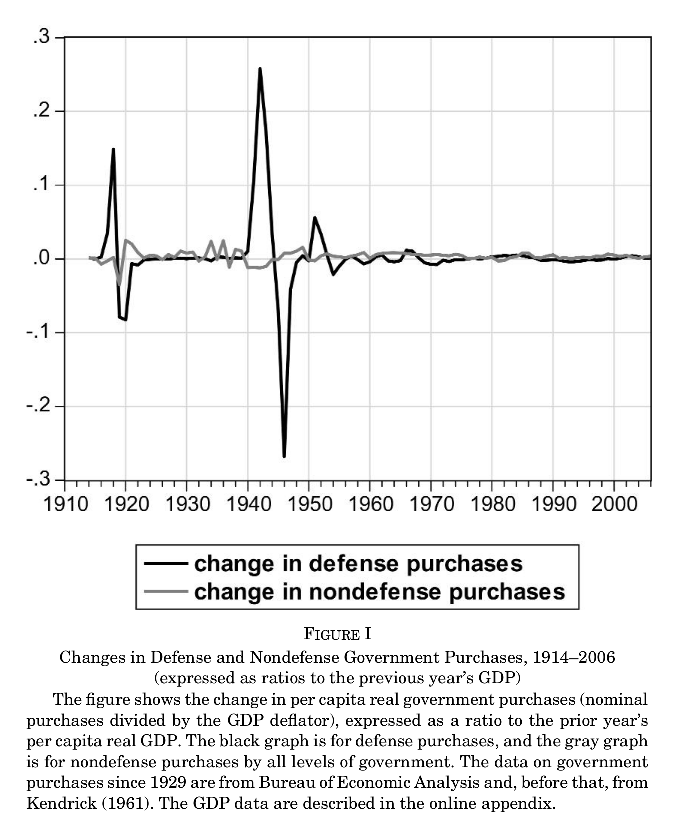
\includegraphics[scale=.5]{barro_redlick1.eps}
  \end{figure}
  Barro \& Redlick, 2011
\end{frame}
%--------------------------------------

%--------------------------------------
\begin{frame}
  \begin{figure}
    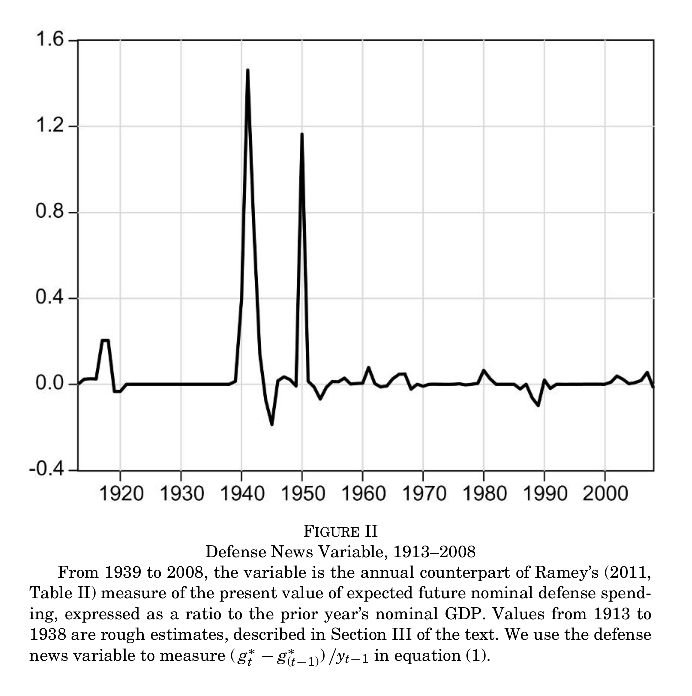
\includegraphics[scale=.5]{barro_redlick2.eps}
  \end{figure}
  Barro \& Redlick, 2011
\end{frame}
%--------------------------------------

%--------------------------------------
\begin{frame}
  \begin{figure}
    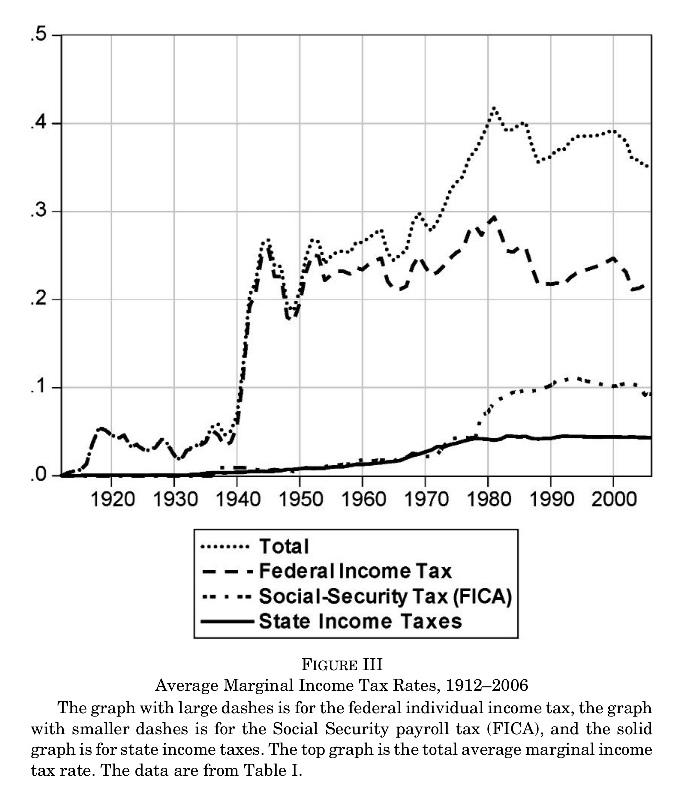
\includegraphics[scale=.5]{barro_redlick3.eps}
  \end{figure}
  Barro \& Redlick, 2011
\end{frame}
%--------------------------------------

%--------------------------------------
\begin{frame}
  \begin{figure}
    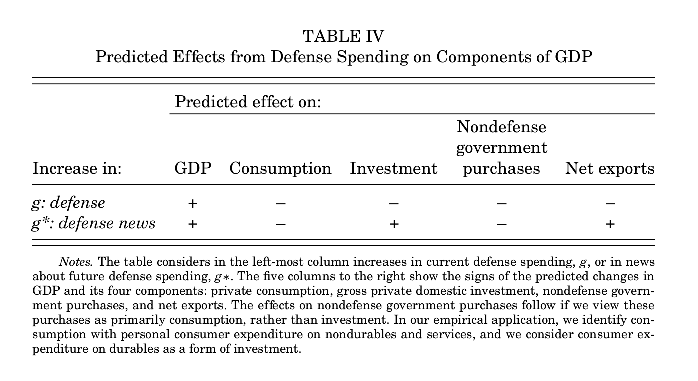
\includegraphics[scale=.5]{barro_redlick4.eps}
  \end{figure}
  Barro \& Redlick, 2011
\end{frame}
%--------------------------------------

%--------------------------------------
\begin{frame}
 Let's turn the attention to evidence for the non-neutrality of monetary policy. 
 Nakamura \& Steinsson highlight three prominent pieces of evidence
 \begin{enumerate}
   \item Bad policy by the FED prior to the Great Depression which made things worse
   \item the Volcker disflation
   \item Break in volatility of US real exchange rate
 \end{enumerate} 
\end{frame}
%--------------------------------------

%--------------------------------------
\begin{frame}
  \begin{figure}
    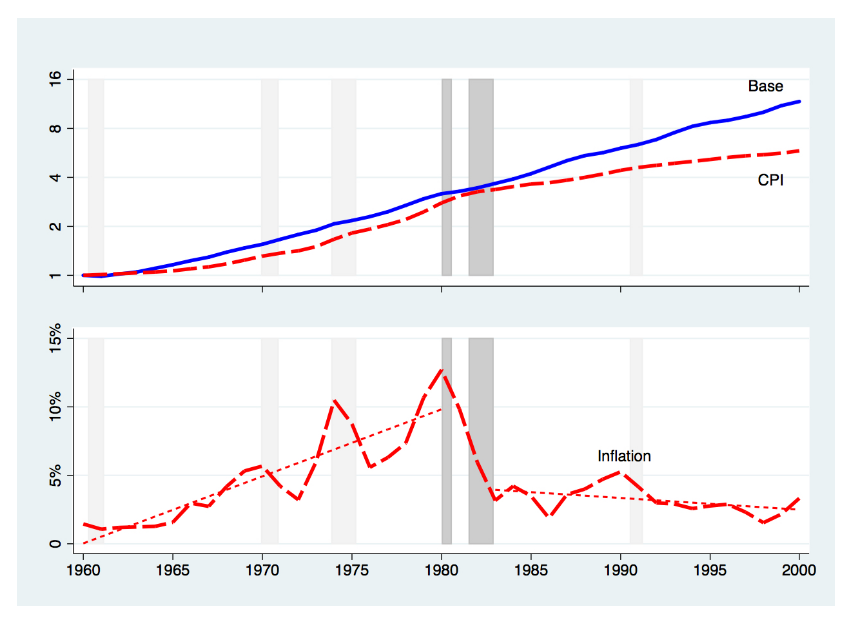
\includegraphics[scale=.7]{romer.eps}
  \end{figure}
  Romer (2016)
\end{frame}
%--------------------------------------


%--------------------------------------
\begin{frame}
  \begin{figure}
    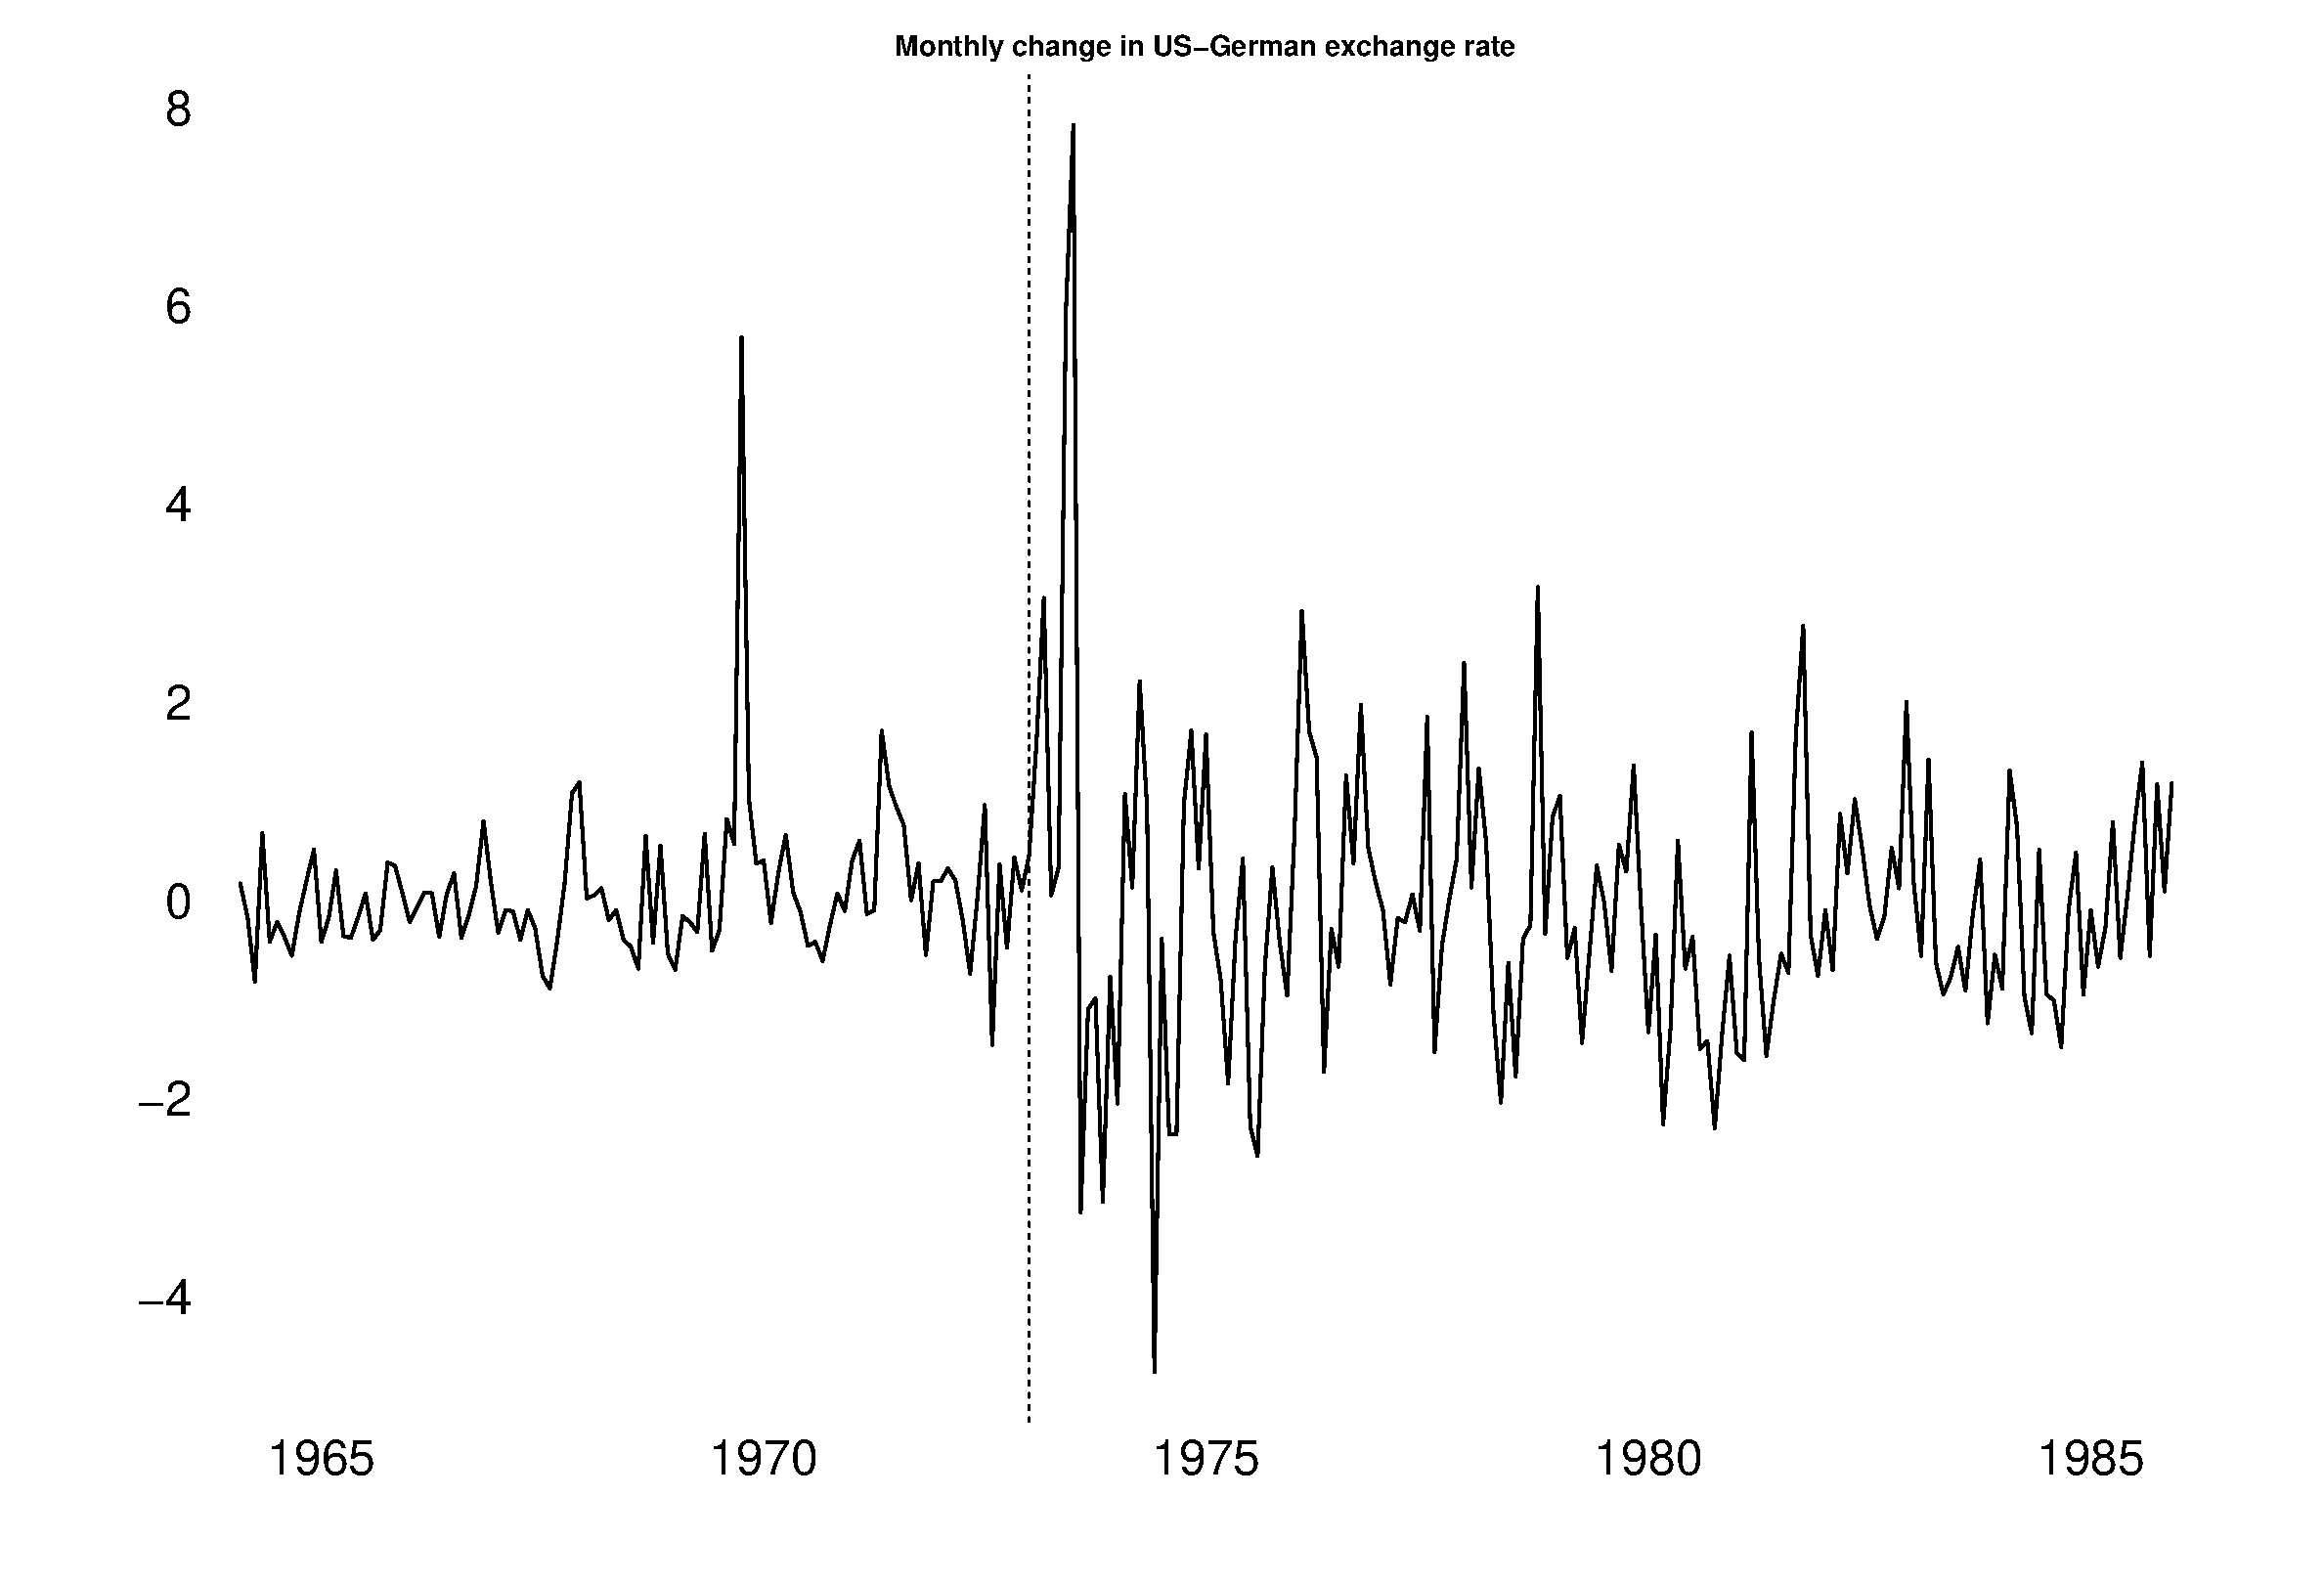
\includegraphics[scale=.3]{exchange_rate.eps}
  \end{figure}  
\end{frame}
%--------------------------------------


%--------------------------------------
\begin{frame}
  Provided evidence gives a glimpse into preferred empirical methods
  \begin{itemize}
    \item Two cases are exclusively based on historical events
    \item One is example of identification based on discontinuity
  \end{itemize}
  \medskip
  Not appearing in this list: VARs
\end{frame}
%--------------------------------------

%--------------------------------------
\begin{frame}
  Four prevalent approaches
  \begin{enumerate}
    \item Large shocks
    \item Discontinuity-based identification
    \item Narrative record to identify shocks
    \item 'Controlling' for confounding factors
  \end{enumerate}
\end{frame}
%--------------------------------------





\end{document}
